\usetikzlibrary{arrows.meta}
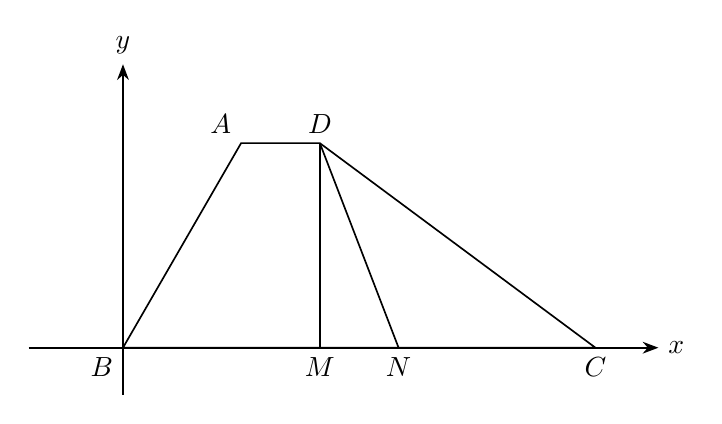
\begin{tikzpicture}[x=1cm,y=1cm,line width=.6pt,font=\normalsize,>=Stealth]
\coordinate (B) at (0,0);
\coordinate (A) at (1.5,2.5980762114);
\coordinate (D) at (2.5,2.5980762114);
\coordinate (C) at (6,0);
\coordinate (M) at (2.5,0);
\coordinate (N) at (3.5,0);
\coordinate (XMIN) at (-1.2,0);
\coordinate (XMAX) at (6.8,0);
\coordinate (YMIN) at (0,-0.6);
\coordinate (YMAX) at (0,3.6);
\draw[->] (XMIN)--(XMAX) node[right] {$x$};
\draw[->] (YMIN)--(YMAX) node[above] {$y$};
\draw (B)--(A)--(D)--(C)--cycle;
\draw (D)--(M);
\draw (D)--(N);
\node[below left] at (B) {$B$};
\node[above left] at (A) {$A$};
\node[above] at (D) {$D$};
\node[below] at (M) {$M$};
\node[below] at (N) {$N$};
\node[below] at (C) {$C$};
\end{tikzpicture}
